\chapter{Deep, Interpretable Knowledge Tracing Methods} \label{ch:kt_methods}

The deep neural network approaches described in the previous section (including DKT, DKVMN, and SAKT) to the knowledge tracing problem have produced very high predictive power. Given a sequence of previous student interactions and a current question, they are capable of outputting the probability that the current question will be answered correctly with high accuracy. For the most part, this is the only metric produced by these models to measure student learning. But there already exists a theoretical framework for computing the probability of a correct response: Item Response Theory, introduced in Section \ref{sec:irt}.

In this section, we introduce an interpretable modification to deep knowledge tracing methods, published in the proceedings of AIED 2021 \cite{kt_irt}. Specifically, we link Item Response Theory models into the structure of knowledge tracing neural architecture. Besides the theoretical advantages this gives to a knowledge tracing model, it is also very helpful in practice. First, it provides an accessible and explicit representation of student knowledge at each timestep. This is an upgrade from other deep knowledge tracing methods, where the only meaningful values produced is $p_{t+1}$, the probability of answering the next question correctly (Equation \ref{eq:kt_prob}). The proposed modification also functions as a parameter estimation technique, quantifying the difficulty and discrimination power of items.

The connection between knowledge tracing and IRT has been explored before via Deep-IRT. The IRT-inspired knowledge tracing methods presented here differ from Deep-IRT in a few ways. First, Deep-IRT is tightly coupled with DKVMN, while the proposed method is readily applicable to a variety of deep knowledge tracing models. Our approach also allows for items to be associated with multiple skills, and directly emulates the ML2P model in Equation \ref{eq:ml2p} or the Rasch model in Equation \ref{eq:rasch} by producing estimates to discrimination and difficulty parameters. The focus here involves item-level parameters, rather than the concept-level parameters considered in Deep-IRT. The implementation details we use are completely different from that of Deep-IRT. Rather than adding separate networks for each parameter, we modify the output layer using information from the item-skill association $Q$-matrix, similar to the methodology of ML2P-VAE in Section \ref{sec:ml2p_vae}.

In this chapter, a trade-off is presented between predictive power and interpretability, but the proposed method remains competitive with other deep learning methods. While sacrificing a small amount of accuracy (measured by AUC), IRT-inspired knowledge tracing provides an explicit representation of student knowledge $\vect \Theta$ at each timestep. This representation of student knowledge is an upgrade from other deep knowledge tracing methods, which approximate skill mastery after the fact by averaging the probability of correctly answering all items associated with a particular skill. Additionally, parameters of the proposed modified neural network can be interpreted as approximations to the item parameters $a_{ik}$ and $b_i$ in Equation \ref{eq:ml2p}. In this sense, our proposed models function as both a knowledge tracing and a parameter estimation method.


\section{Incorporating IRT into Knowledge Tracing} \label{sec:kt_irt_methods}
Given a tutoring system with $n$ available items, $K$ skills under assessment, and the skill association of each item given as a binary matrix $Q \in \{0,1\}^{n \times K}$ \cite{daSilva2018}, each of the possible $2n$ student interactions $(q_t, c_t)$ is represented as a learned $d$-dimensional vector $\vect x_t \in \mathbb{R}^d$. This can be done by multiplying a one-hot encoding of the $2n+1$ interactions (including a null/padding interaction) by a trainable $(2n+1) \times d$ matrix.

Each student's response sequence includes $\vect x_0$, a null interaction to indicate the start of their interactions. A hyper-parameter $L$ is chosen indicating the maximum length of a student's response sequence. Interaction sequences shorter than $L$ are padded, and interaction sequences longer than $L$ are split into multiple sequences. A student's sequence of embedded interactions $\{\vect x_t\}_{t=0}^L$ is fed through a temporal neural network (TNN), such as an LSTM (similar to DKT \cite{piech2015}) or an attention-based model (similar to SAKT \cite{pandey2019}). This outputs an $h$-dimensional vector $\vect v_t$ for each interaction $\vect x_t$ in the input sequence.

\begin{equation}
  \vect v_t = \text{TNN}(\vect x_t, \vect x_{t-1}, \ldots, \vect x_0), \quad \vect v_t \in \R^h
  \label{eq:tsnn_layer}
\end{equation}

Next, each $\vect v_t$ is sent through a linear layer feed-forward network with output size $K$ (the number of latent concepts), yielding the skill vector $\vect s_t$.
\begin{equation}
  \vect s_t = W_s \vect v_t + \vect y, \quad W_s \in \R^{K\times h}, \vect y \in \R^K
  \label{eq:skill_layer}
\end{equation}
The weights matrix $W_s$ and bias vector $\vect y$ are trainable parameters. Each node in this ``skill layer'' represents a knowledge concept.

Finally, the output layer of the model has $n$ nodes and a sigmoid activation function $\sigma(\cdot)$, with each node representing the probability of the student answering that item correctly.

\begin{equation}
  \vect p_t = \sigma(W_p \vect s_t + \vect z) = \frac{1}{1 + \exp \left( -W_p \vect s_t - \vect z \right)}, \quad W_p \in \R^{n \times K}, \vect z \in \R^n.
  \label{eq:pred_layer}
\end{equation}
$W_p$ and $\vect z$ are trainable and importantly, $W_p$ is modified so that the nonzero values of $W_p$ are determined by the $Q$-matrix \cite{guo2017}\cite{ijcnn_paper}. If item $i$ does not require skill $k$, then the weight between the corresponding nodes is fixed to be zero. In this way, we write
\begin{equation}
  W_p \gets W_p \odot Q,
  \label{eq:weight_constraint}
\end{equation}
where $\odot$ is element-wise multiplication of matrices. Then the probability that the student will answer question $i$ correctly at timestep $t$ is given by 
\begin{equation}
  p_{ti} = \frac{1}{1 + \exp\left( -\sum_{k=1}^K w_{ik} q_{ik} s_{tk} - z_i \right)}
  \label{eq:nn_out}
\end{equation}
where $w_{ik}$, $q_{ik}$, $s_{tk}$, and $z_i$ are entries in $W_p$, $Q$, $\vect s_t$, and $\vect z$, respectively.

\begin{figure}[h]
  \centering
  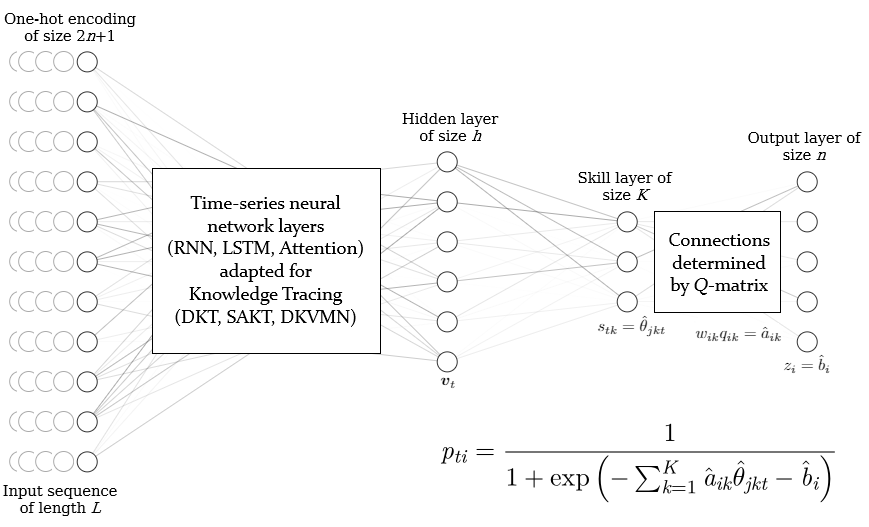
\includegraphics[width=.95\textwidth]{img/kt_irt/kt_irt_visual_with_equation_2.png}
  \caption{Visualization of integrating IRT into a knowledge tracing model with $L=4$, $n=5$, and $K=3$.}
  \label{fig:kt_irt_visual}
\end{figure}

This constraint allows for interpretation of the final neural network layers as an approximate ML2P model: note the similarity between Equation \ref{eq:nn_out} and Equation \ref{eq:ml2p}. A visualization of this proposed neural network architecture is seen in Figure \ref{fig:kt_irt_visual}.

%\begin{figure}[h]
%  \centering
%  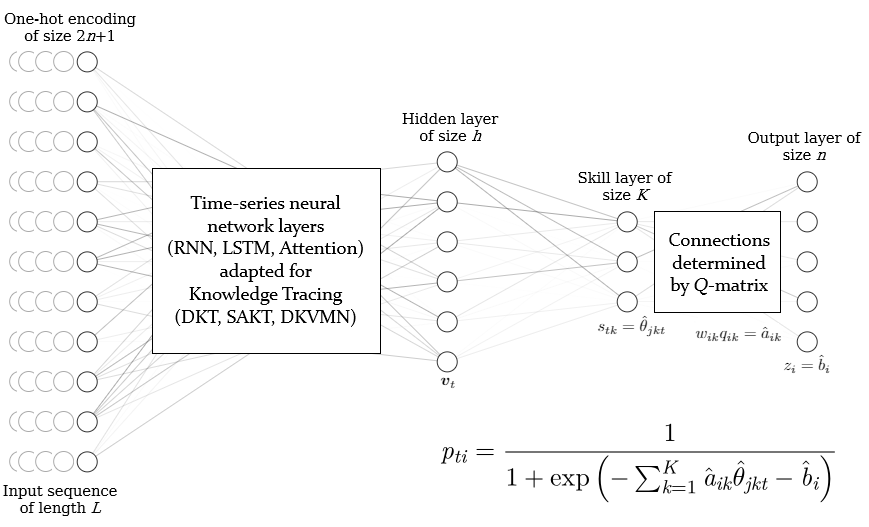
\includegraphics[width=.95\textwidth]{img/kt_irt/kt_irt_visual_with_equation_2.png}
%  \caption{Visualization of integrating IRT into a knowledge tracing model with $L=4$, $n=5$, and $K=3$.}
%  \label{fig:kt_irt_visual}
%\end{figure}

The weights between the skill and output layer $(w_{ik}q_{ik})$ serve as estimates to the discrimination parameters $a_{ik}$, and the bias parameters in the output layer $z_i$ are estimates to difficulty parameters $b_i$. The student's $k$-th latent ability $\theta_k$ is estimated at timestep $t$ via $s_{tk}$. This presents a clear analogue with ML2P-VAE, but the method described in this section makes no assumption about the prior distribution of latent traits $\vect \Theta$ -- there is no KL-Divergence term in the knowledge tracing loss function. In this way, IRT-inspired knowledge tracing is more similar to the modified autoencoder proposed by Guo et al. \cite{guo2017} and described in Section \ref{sec:ae_v_vae_results}.

